
\section{Introduction}

  Comparison of extremely high dimensional data using direct methods has shown to be
  too computationally expensive and inaccurate.  By transforming the data to a
  customized, low dimensional space; constructed solely to represent one particular
  type of data; a faster, more accurate comparison can be made.  This new space can
  be formed using a method known as Principal Component Analysis (PCA).  PCA determines
  a basis for a lower dimensional space by calculating the eigenvectors and eigenvalues
  of the covariance matrix. The covariance matrix is a special matrix constructed
  from data in a set containing one particular type of data. The eigenvectors which
  correspond to the largest eigenvalues are then kept to form a basis. It has been shown
  that using this method, the dimensionality of the data to be significantly reduced,
  while retaining nearly all of the information.

  For the eigenface approach, the space which represents the vectors are is constructed with
  the sole intent of representing faces.  This is done by taking a large database of face
  images, representing them as vectors, then using PCA to form a new basis.  The basis
  vectors are known as eigenfaces because they are eigenvectors yet resemble faces.  Some
  of these eigenfaces can be seen in Fig.~\ref{fig:top_efaces}.  From now on, the space
  defined by the eigenfaces will be known as the eigenspace.

  Every face in the database can be represented as a linear combination of the eigenfaces.
  The coefficients in this linear combination are the new vectors used to represent the
  various faces.  Other images may also be transformed into the eigenspace, under the
  constraint that they are the same size as the original images from the database.

\section{Datasets}

  For the experiments, two datasets are used, a training set containing 1204 faces from 867
  subjects, and a testing set containing 1196 faces from 866 subjects. All 866 subjects
  from the testing dataset exist in the training database (i.e., there is one extra
  subject in the training set).  A truncated training set is used in the second experiment
  where the images of the first 50 subjects are removed (i.e., the testing set contains
  50 subjects that do not exist in the training set).  Each dataset exists at two
  resolutions, $48 \times 60$ and $16 \times 20$, all experiments were done at both high
  and low resolutions.
  
\section{Experiments}

  The first experiment attempts to obtain the identity of a face using the eigenspace
  approach.  The eigenspace is constructed using the 1204 faces from the training set.
  The faces from the testing set are then transformed into the eigenspace and compared
  to the training faces.  This comparison is done using the Malahanobis distance 
  (Eq.~\ref{eq:mal}) rather than the Euclidean distance.  The Malahanobis distance
  allows variations along all axes to be treated as equally significant.  If the correct
  identification is found among the top $N$ matches, then the match was successful.  By
  varying $N$ from $1$ to $50$, and recording the accuracy across the entire testing set,
  the CMC graph is obtained.  This is used to represent the matching power of the
  algorithm.  This experiment is repeated three times using eigenspaces constructed to
  retain 80\%, 90\%, and 95\% of the information from the training set.

  \begin{equation}
    \sum_{i=1}^K {1 \over \lambda_i} (w_i - w_i^l)^2
    \label{eq:mal}
  \end{equation}

  The second experiment attempts to detect intruders in the test set.  This is done by
  using a training set with the first 50 subjects removed.  The eigenspace is then
  constructed using 95\% information retention.  Each face from the test set is compared
  to each face in the training set and the smallest Malahanobis distance score is found
  (Eq.~\ref{eq:mal}).  If this score is above a particular threshold the face is
  rejected as an intruder.  By using many different thresholds, the ROC curve is found
  which represents this methods ability to reject intruders while retaining non-intruders.

\section{Results}

  \subsection{Face Identification}

  The CMC graph for the high-resolution dataset (Fig.~\ref{fig:cmc_h}) shows that using
  all three eigenspaces give similar results.  The 90\% eigenspace seems to yield the best
  results, however the 80\% eigenspace gives nearly identical results once $N$ becomes
  larger than $25$.  The 95\% eigenspace is similar the the 90\% eigenspace when $N$ is
  less than $5$, but quickly diverges and maintains a 4\% less recognition rate for larger
  $N$.  Based on these results, 90\% gives the best results, but if speed is a factor, 80\%
  gives very similar results as well.

  These results seem to signify that most of the important information needed for high-level
  comparison is in the first coefficients.  If too many are used then useless information is
  introduced and performance begin to deteriorate.  Examples of correctly matched faces,
  along with top matches from the training set can be seen in Figs.~\ref{fig:correct80},
  ~\ref{fig:correct90}, and~\ref{fig:correct95}.  The left-most image is the test face, and
  the following faces to the right are the best matched faces from the training set.  The
  largest of these right-most faces indicate correct matches.  Examples of incorrectly
  matched faces can be seen in Figs.~\ref{fig:incorrect80},~\ref{fig:incorrect90}, and
  ~\ref{fig:incorrect95} along with the ten best matches where non of these are the
  correct match.

  The CMC graph for the low-resolution dataset (Fig.~\ref{fig:cmc_l}) shows that perhaps
  80\% information retention is not good enough for low-resolution images.  This graph
  also shows an improvement of approximately $2-5\%$ for the 90\% and 95\% eigenspaces.
  This result is counter-intuitive because people generally find it more difficult to
  identify a person from a low resolution image.  A possible explanation of this
  phenomenon is that, at lower resolutions, only large defining features are kept.  This
  allows insignificant information such as some lighting conditions and noise to be
  less invasive.

  \subsection{Intruder Detection}

  The ROC generated by testing many thresholds in the high-resolution dataset
  (Fig.~\ref{fig:roc_h}) appears to accept approximately 25\% of intruders while retaining
  70\% of non-intruders. Although this ratio is not great, this method definitely has
  some intruder detection abilities.  By setting a high threshold, 90\% of of non-intruders
  are accepted and 50\% of intruders are accepted.  By using this high threshold, it may
  be possible to make this a part of a cascade detection system which could use this as
  one of multiple steps in intruder detection.
  
  At low-resolution (Fig.~\ref{fig:roc_l}, the rejection/acceptance rate is nearly identical.
  This implies that using high-resolution images is not beneficial and should therefore
  not be done because low-resolution images allow for faster calculations with no observable
  negative effects.

\section{Questions}

\begin{enumerate}

  \item What is dimensionality reduction and why is it important?

  \begin{enumerate}
    \item Dimensionality reduction reduces the number of coefficients required to
          represent a vector.  This is important because it reduces the processing
          time for any computation on the vector.
  \end{enumerate}

  \item What is the criterion used by PCA for determining a space of low dimensionality?

  \begin{enumerate}
    \item Find a basis that includes only the vectors which allow for the greatest information retention.
  \end{enumerate}

  \item How is the lower dimensionality space computed using PCA?

  \begin{enumerate}
    \item Form the lower dimensionality basis from the top $K$ eigenvectors of the
          covariance matrix $C$, where $C$ is calculated using the following formula.

    Assume $x_1, x_2, ..., x_M$ are column vectors and $|x_i|=N$
    \begin{enumerate}
      \item $\overline{x} = {1 \over M} \sum_{i=1}^M x_i$
      \item $\Phi_i = x_i - \overline{x}$
      \item form the matrix $A = [\Phi_1 \Phi_2 \cdots \Phi_M]$ \hspace{10pt} $(A$ is an $N \times M$ matrix)
      \\

      $C = {1 \over M} \sum_{n=1}^M \Phi_n \Phi_n^T = {1 \over M} AA^T$
    \end{enumerate}
  \end{enumerate}

  \item What is the geometrical interpretation of PCA?

  \begin{enumerate}
    \item The eigenvectors used to form the basis represent the axes where the data in $x$ varies the most.
          The axes where the data varies the least represents the least information and is therefore removed.
  \end{enumerate}

  \item How do we choose the number of dimensions?

  \begin{enumerate}
    \item After determining the amount of data to preserve, PCA takes the top $K$
          eigenvectors of $AA^T$ where $K$ is the minimum number of eigenvalues $\lambda_i$
          of $AA^T$ required to meet the following formula.

          \[
            {\sum_{i=1}^K \lambda_i \over \sum_{i=1}^N \lambda_i} > T
          \]

          Where $0 < T \leq 1$ is the minimum amount of data to preserve.
  \end{enumerate}

  \item What are the steps for face recognition using PCA?

  \begin{enumerate}
    \item Take each $N \times N$ face image and in the training set and turn it into an $N^2$ column vector $x_i$ then use PCA to reduce the
          dimensionality of $x_i$ from $N^2$ to $K$ where $\Omega_i^l$ are the reduced vectors
          , $\Psi$ is the mean face, and $u_i$ are the basis eigenvectors.
    \begin{enumerate}
      \item Normalize $\Gamma: \Phi = \Gamma - \Psi$
      \item Project $\Psi$ onto the eigenspace: $\Omega = [w_1 w_2 \cdots w_3]^T$ \hspace{15pt} $(w_i = u_i^T \Phi)$
      \item compute $e_r = min\left \| \Omega - \Omega_i^l \right \|$ using the Mahalanobis distance.
      \item if $e_r < Threshold$ then $\Gamma$ is a face, otherwise it is not.
    \end{enumerate}
  \end{enumerate}

\end{enumerate}

\clearpage

\section{Images}

%\begin{figure}[hbt]
%  \centering
%  \subfigure[CAP]{
%    \includegraphics[width=0.4\textwidth]{}
%  }
%  \caption{}
%  % Put the label at the bottom
%  \label{fig:}
%\end{figure}

\begin{figure}[hbt]
  \centering
  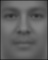
\includegraphics[width=0.25\textwidth]{../results/H_rez/mean_face.jpg}
  \caption{Average face}
  \label{fig:mean}
\end{figure}

~\vfill

\begin{figure}[hbt]
  \centering
  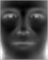
\includegraphics[width=0.18\textwidth]{../results/H_rez/eigenfaces/largest1.jpg}
  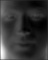
\includegraphics[width=0.18\textwidth]{../results/H_rez/eigenfaces/largest2.jpg}
  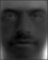
\includegraphics[width=0.18\textwidth]{../results/H_rez/eigenfaces/largest3.jpg}
  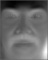
\includegraphics[width=0.18\textwidth]{../results/H_rez/eigenfaces/largest4.jpg}
  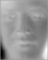
\includegraphics[width=0.18\textwidth]{../results/H_rez/eigenfaces/largest5.jpg} \\
  \vspace{4pt}
  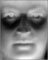
\includegraphics[width=0.18\textwidth]{../results/H_rez/eigenfaces/largest6.jpg}
  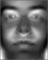
\includegraphics[width=0.18\textwidth]{../results/H_rez/eigenfaces/largest7.jpg}
  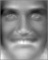
\includegraphics[width=0.18\textwidth]{../results/H_rez/eigenfaces/largest8.jpg}
  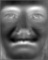
\includegraphics[width=0.18\textwidth]{../results/H_rez/eigenfaces/largest9.jpg}
  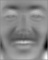
\includegraphics[width=0.18\textwidth]{../results/H_rez/eigenfaces/largest10.jpg}
  \caption{Top ten Eigenfaces}
  \label{fig:top_efaces}
\end{figure}

~\vfill

\begin{figure}[hbt]
  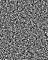
\includegraphics[width=0.09\textwidth]{../results/H_rez/eigenfaces/smallest1.jpg}
  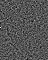
\includegraphics[width=0.09\textwidth]{../results/H_rez/eigenfaces/smallest2.jpg}
  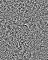
\includegraphics[width=0.09\textwidth]{../results/H_rez/eigenfaces/smallest3.jpg}
  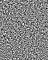
\includegraphics[width=0.09\textwidth]{../results/H_rez/eigenfaces/smallest4.jpg}
  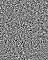
\includegraphics[width=0.09\textwidth]{../results/H_rez/eigenfaces/smallest5.jpg}
  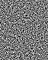
\includegraphics[width=0.09\textwidth]{../results/H_rez/eigenfaces/smallest6.jpg}
  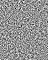
\includegraphics[width=0.09\textwidth]{../results/H_rez/eigenfaces/smallest7.jpg}
  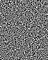
\includegraphics[width=0.09\textwidth]{../results/H_rez/eigenfaces/smallest8.jpg}
  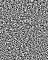
\includegraphics[width=0.09\textwidth]{../results/H_rez/eigenfaces/smallest9.jpg}
  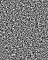
\includegraphics[width=0.09\textwidth]{../results/H_rez/eigenfaces/smallest10.jpg}
  \caption{Bottom ten Eigenfaces}
  \label{fig:bot_efaces}
\end{figure}

~\vfill

\vfill

~\vfill

\begin{figure}[hbt]
  \centering
  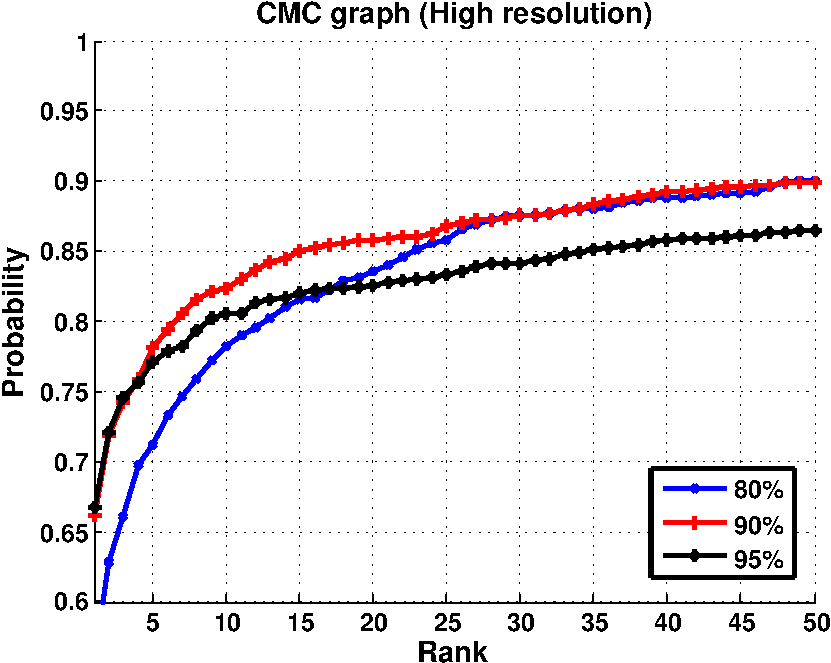
\includegraphics[width=0.7\textwidth]{../results/Output_H.pdf}
  \caption{High resolution CMC for training at 80\%, 90\%, and 95\% information retention.}
  \label{fig:cfc_h}
\end{figure}

~\vfill

\begin{figure}[hbt]
  \centering
  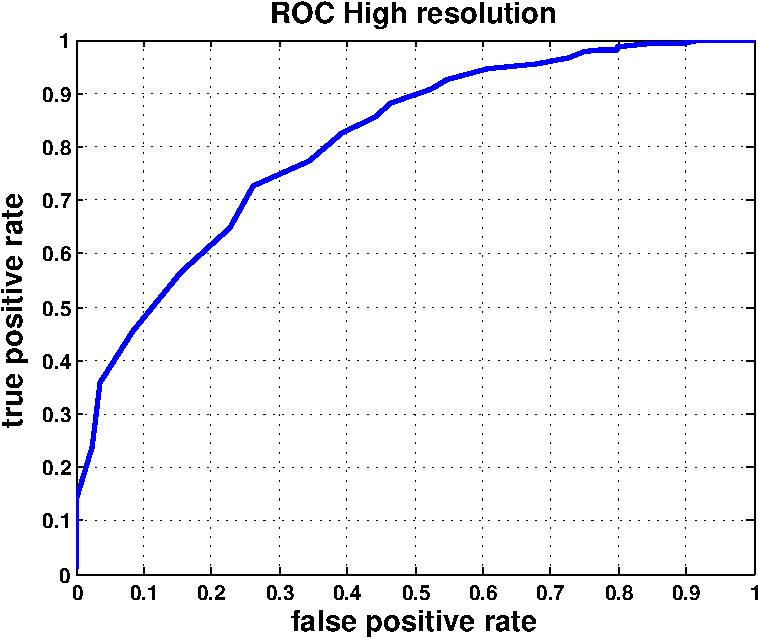
\includegraphics[width=0.7\textwidth]{../results/ROC_H.pdf}
  \caption{High resolution ROC.}
  \label{fig:roc_h}
\end{figure}

~\vfill

\vfill

~\vfill

\begin{figure}[hbt]
  \centering
  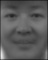
\includegraphics[width=0.1\textwidth]{../results/H_rez/correct80/1/testImg.jpg} \vline
  \hspace{2pt}
  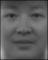
\includegraphics[width=42pt]{../results/H_rez/correct80/1/1.jpg}
  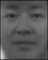
\includegraphics[width=42pt]{../results/H_rez/correct80/1/2.jpg}
  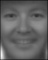
\includegraphics[width=31pt]{../results/H_rez/correct80/1/3.jpg}
  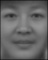
\includegraphics[width=42pt]{../results/H_rez/correct80/1/4.jpg}
  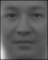
\includegraphics[width=31pt]{../results/H_rez/correct80/1/5.jpg}
  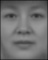
\includegraphics[width=31pt]{../results/H_rez/correct80/1/6.jpg}
  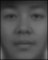
\includegraphics[width=42pt]{../results/H_rez/correct80/1/7.jpg}
  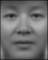
\includegraphics[width=42pt]{../results/H_rez/correct80/1/8.jpg}
  
\includegraphics[width=31pt]{../results/H_rez/correct80/1/9.jpg}
  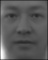
\includegraphics[width=31pt]{../results/H_rez/correct80/1/10.jpg} \\
  \vspace{4pt}
  
\includegraphics[width=0.1\textwidth]{../results/H_rez/correct80/2/testImg.jpg} \vline
  \hspace{2pt}
  
\includegraphics[width=0.09\textwidth]{../results/H_rez/correct80/2/1.jpg}
  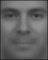
\includegraphics[width=0.09\textwidth]{../results/H_rez/correct80/2/2.jpg}
  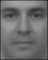
\includegraphics[width=0.07\textwidth]{../results/H_rez/correct80/2/3.jpg}
  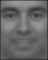
\includegraphics[width=0.09\textwidth]{../results/H_rez/correct80/2/4.jpg}
  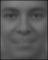
\includegraphics[width=0.07\textwidth]{../results/H_rez/correct80/2/5.jpg}
  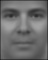
\includegraphics[width=0.09\textwidth]{../results/H_rez/correct80/2/6.jpg}
  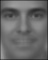
\includegraphics[width=0.07\textwidth]{../results/H_rez/correct80/2/7.jpg}
  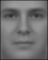
\includegraphics[width=0.07\textwidth]{../results/H_rez/correct80/2/8.jpg}
  
\includegraphics[width=0.07\textwidth]{../results/H_rez/correct80/2/9.jpg}
  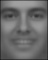
\includegraphics[width=0.07\textwidth]{../results/H_rez/correct80/2/10.jpg} \\
  \vspace{4pt}
  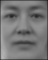
\includegraphics[width=0.1\textwidth]{../results/H_rez/correct80/3/testImg.jpg} \vline
  \hspace{2pt}
  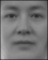
\includegraphics[width=0.09\textwidth]{../results/H_rez/correct80/3/1.jpg}
  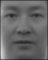
\includegraphics[width=0.07\textwidth]{../results/H_rez/correct80/3/2.jpg}
  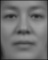
\includegraphics[width=0.09\textwidth]{../results/H_rez/correct80/3/3.jpg}
  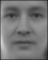
\includegraphics[width=0.07\textwidth]{../results/H_rez/correct80/3/4.jpg}
  \includegraphics[width=0.09\textwidth]{../results/H_rez/correct80/3/5.jpg}
  \includegraphics[width=0.07\textwidth]{../results/H_rez/correct80/3/6.jpg}
  \includegraphics[width=0.07\textwidth]{../results/H_rez/correct80/3/7.jpg}
  \includegraphics[width=0.07\textwidth]{../results/H_rez/correct80/3/8.jpg}
  \includegraphics[width=0.07\textwidth]{../results/H_rez/correct80/3/9.jpg}
  \includegraphics[width=0.09\textwidth]{../results/H_rez/correct80/3/10.jpg}
  \caption{Top matches for 3 correctly matched faces at 80\% information retention.}
  \label{fig:correct80}
\end{figure}

~\vfill

\begin{figure}[hbt]
  \centering
  \includegraphics[width=0.1\textwidth]{../results/H_rez/incorrect80/1/testImg.jpg} \vline
  \hspace{2pt}
  \includegraphics[width=0.08\textwidth]{../results/H_rez/incorrect80/1/1.jpg}
  \includegraphics[width=0.08\textwidth]{../results/H_rez/incorrect80/1/2.jpg}
  \includegraphics[width=0.08\textwidth]{../results/H_rez/incorrect80/1/3.jpg}
  \includegraphics[width=0.08\textwidth]{../results/H_rez/incorrect80/1/4.jpg}
  \includegraphics[width=0.08\textwidth]{../results/H_rez/incorrect80/1/5.jpg}
  \includegraphics[width=0.08\textwidth]{../results/H_rez/incorrect80/1/6.jpg}
  \includegraphics[width=0.08\textwidth]{../results/H_rez/incorrect80/1/7.jpg}
  \includegraphics[width=0.08\textwidth]{../results/H_rez/incorrect80/1/8.jpg}
  \includegraphics[width=0.08\textwidth]{../results/H_rez/incorrect80/1/9.jpg}
  \includegraphics[width=0.08\textwidth]{../results/H_rez/incorrect80/1/10.jpg} \\
  \vspace{4pt}
  \includegraphics[width=0.1\textwidth]{../results/H_rez/incorrect80/2/testImg.jpg} \vline
  \hspace{2pt}
  \includegraphics[width=0.08\textwidth]{../results/H_rez/incorrect80/2/1.jpg}
  \includegraphics[width=0.08\textwidth]{../results/H_rez/incorrect80/2/2.jpg}
  \includegraphics[width=0.08\textwidth]{../results/H_rez/incorrect80/2/3.jpg}
  \includegraphics[width=0.08\textwidth]{../results/H_rez/incorrect80/2/4.jpg}
  \includegraphics[width=0.08\textwidth]{../results/H_rez/incorrect80/2/5.jpg}
  \includegraphics[width=0.08\textwidth]{../results/H_rez/incorrect80/2/6.jpg}
  \includegraphics[width=0.08\textwidth]{../results/H_rez/incorrect80/2/7.jpg}
  \includegraphics[width=0.08\textwidth]{../results/H_rez/incorrect80/2/8.jpg}
  \includegraphics[width=0.08\textwidth]{../results/H_rez/incorrect80/2/8.jpg}
  \includegraphics[width=0.08\textwidth]{../results/H_rez/incorrect80/2/10.jpg} \\
  \vspace{4pt}
  \includegraphics[width=0.1\textwidth]{../results/H_rez/incorrect80/3/testImg.jpg} \vline
  \hspace{2pt}
  \includegraphics[width=0.08\textwidth]{../results/H_rez/incorrect80/3/1.jpg}
  \includegraphics[width=0.08\textwidth]{../results/H_rez/incorrect80/3/2.jpg}
  \includegraphics[width=0.08\textwidth]{../results/H_rez/incorrect80/3/3.jpg}
  \includegraphics[width=0.08\textwidth]{../results/H_rez/incorrect80/3/4.jpg}
  \includegraphics[width=0.08\textwidth]{../results/H_rez/incorrect80/3/5.jpg}
  \includegraphics[width=0.08\textwidth]{../results/H_rez/incorrect80/3/6.jpg}
  \includegraphics[width=0.08\textwidth]{../results/H_rez/incorrect80/3/7.jpg}
  \includegraphics[width=0.08\textwidth]{../results/H_rez/incorrect80/3/8.jpg}
  \includegraphics[width=0.08\textwidth]{../results/H_rez/incorrect80/3/8.jpg}
  \includegraphics[width=0.08\textwidth]{../results/H_rez/incorrect80/3/10.jpg}
  \caption{Top matches for 3 incorrectly matched faces at 80\% information retention.}
  \label{fig:incorrect80}
\end{figure}

~\vfill

\clearpage

~\vfill

\begin{figure}[hbt]
  \centering
  \includegraphics[width=0.1\textwidth]{../results/H_rez/correct90/1/testImg.jpg} \vline
  \hspace{2pt}
  \includegraphics[width=0.09\textwidth]{../results/H_rez/correct90/1/1.jpg}
  \includegraphics[width=0.09\textwidth]{../results/H_rez/correct90/1/2.jpg}
  \includegraphics[width=0.09\textwidth]{../results/H_rez/correct90/1/3.jpg}
  \includegraphics[width=0.09\textwidth]{../results/H_rez/correct90/1/4.jpg}
  \includegraphics[width=0.06\textwidth]{../results/H_rez/correct90/1/5.jpg}
  \includegraphics[width=0.09\textwidth]{../results/H_rez/correct90/1/6.jpg}
  \includegraphics[width=0.06\textwidth]{../results/H_rez/correct90/1/7.jpg}
  \includegraphics[width=0.09\textwidth]{../results/H_rez/correct90/1/8.jpg}
  \includegraphics[width=0.06\textwidth]{../results/H_rez/correct90/1/9.jpg}
  \includegraphics[width=0.06\textwidth]{../results/H_rez/correct90/1/10.jpg} \\
  \vspace{4pt}
  \includegraphics[width=0.1\textwidth]{../results/H_rez/correct90/2/testImg.jpg} \vline
  \hspace{2pt}
  \includegraphics[width=0.09\textwidth]{../results/H_rez/correct90/2/1.jpg}
  \includegraphics[width=0.09\textwidth]{../results/H_rez/correct90/2/2.jpg}
  \includegraphics[width=0.09\textwidth]{../results/H_rez/correct90/2/3.jpg}
  \includegraphics[width=0.09\textwidth]{../results/H_rez/correct90/2/4.jpg}
  \includegraphics[width=0.09\textwidth]{../results/H_rez/correct90/2/5.jpg}
  \includegraphics[width=0.09\textwidth]{../results/H_rez/correct90/2/6.jpg}
  \includegraphics[width=0.06\textwidth]{../results/H_rez/correct90/2/7.jpg}
  \includegraphics[width=0.06\textwidth]{../results/H_rez/correct90/2/8.jpg}
  \includegraphics[width=0.06\textwidth]{../results/H_rez/correct90/2/8.jpg}
  \includegraphics[width=0.06\textwidth]{../results/H_rez/correct90/2/10.jpg} \\
  \vspace{4pt}
  \includegraphics[width=0.1\textwidth]{../results/H_rez/correct90/3/testImg.jpg} \vline
  \hspace{2pt}
  \includegraphics[width=0.09\textwidth]{../results/H_rez/correct90/3/1.jpg}
  \includegraphics[width=0.09\textwidth]{../results/H_rez/correct90/3/2.jpg}
  \includegraphics[width=0.09\textwidth]{../results/H_rez/correct90/3/3.jpg}
  \includegraphics[width=0.07\textwidth]{../results/H_rez/correct90/3/4.jpg}
  \includegraphics[width=0.07\textwidth]{../results/H_rez/correct90/3/5.jpg}
  \includegraphics[width=0.07\textwidth]{../results/H_rez/correct90/3/6.jpg}
  \includegraphics[width=0.07\textwidth]{../results/H_rez/correct90/3/7.jpg}
  \includegraphics[width=0.07\textwidth]{../results/H_rez/correct90/3/8.jpg}
  \includegraphics[width=0.07\textwidth]{../results/H_rez/correct90/3/8.jpg}
  \includegraphics[width=0.09\textwidth]{../results/H_rez/correct90/3/10.jpg}
  \caption{Top matches for 3 correctly matched faces at 90\% information retention.}
  \label{fig:correct90}
\end{figure}

~\vfill

\begin{figure}[hbt]
  \centering
  \includegraphics[width=0.1\textwidth]{../results/H_rez/incorrect90/1/testImg.jpg} \vline
  \hspace{2pt}
  \includegraphics[width=0.08\textwidth]{../results/H_rez/incorrect90/1/1.jpg}
  \includegraphics[width=0.08\textwidth]{../results/H_rez/incorrect90/1/2.jpg}
  \includegraphics[width=0.08\textwidth]{../results/H_rez/incorrect90/1/3.jpg}
  \includegraphics[width=0.08\textwidth]{../results/H_rez/incorrect90/1/4.jpg}
  \includegraphics[width=0.08\textwidth]{../results/H_rez/incorrect90/1/5.jpg}
  \includegraphics[width=0.08\textwidth]{../results/H_rez/incorrect90/1/6.jpg}
  \includegraphics[width=0.08\textwidth]{../results/H_rez/incorrect90/1/7.jpg}
  \includegraphics[width=0.08\textwidth]{../results/H_rez/incorrect90/1/8.jpg}
  \includegraphics[width=0.08\textwidth]{../results/H_rez/incorrect90/1/9.jpg}
  \includegraphics[width=0.08\textwidth]{../results/H_rez/incorrect90/1/10.jpg} \\
  \vspace{4pt}
  \includegraphics[width=0.1\textwidth]{../results/H_rez/incorrect90/2/testImg.jpg} \vline
  \hspace{2pt}
  \includegraphics[width=0.08\textwidth]{../results/H_rez/incorrect90/2/1.jpg}
  \includegraphics[width=0.08\textwidth]{../results/H_rez/incorrect90/2/2.jpg}
  \includegraphics[width=0.08\textwidth]{../results/H_rez/incorrect90/2/3.jpg}
  \includegraphics[width=0.08\textwidth]{../results/H_rez/incorrect90/2/4.jpg}
  \includegraphics[width=0.08\textwidth]{../results/H_rez/incorrect90/2/5.jpg}
  \includegraphics[width=0.08\textwidth]{../results/H_rez/incorrect90/2/6.jpg}
  \includegraphics[width=0.08\textwidth]{../results/H_rez/incorrect90/2/7.jpg}
  \includegraphics[width=0.08\textwidth]{../results/H_rez/incorrect90/2/8.jpg}
  \includegraphics[width=0.08\textwidth]{../results/H_rez/incorrect90/2/8.jpg}
  \includegraphics[width=0.08\textwidth]{../results/H_rez/incorrect90/2/10.jpg} \\
  \vspace{4pt}
  \includegraphics[width=0.1\textwidth]{../results/H_rez/incorrect90/3/testImg.jpg} \vline
  \hspace{2pt}
  \includegraphics[width=0.08\textwidth]{../results/H_rez/incorrect90/3/1.jpg}
  \includegraphics[width=0.08\textwidth]{../results/H_rez/incorrect90/3/2.jpg}
  \includegraphics[width=0.08\textwidth]{../results/H_rez/incorrect90/3/3.jpg}
  \includegraphics[width=0.08\textwidth]{../results/H_rez/incorrect90/3/4.jpg}
  \includegraphics[width=0.08\textwidth]{../results/H_rez/incorrect90/3/5.jpg}
  \includegraphics[width=0.08\textwidth]{../results/H_rez/incorrect90/3/6.jpg}
  \includegraphics[width=0.08\textwidth]{../results/H_rez/incorrect90/3/7.jpg}
  \includegraphics[width=0.08\textwidth]{../results/H_rez/incorrect90/3/8.jpg}
  \includegraphics[width=0.08\textwidth]{../results/H_rez/incorrect90/3/8.jpg}
  \includegraphics[width=0.08\textwidth]{../results/H_rez/incorrect90/3/10.jpg}
  \caption{Top matches for 3 incorrectly matched faces at 90\% information retention.}
  \label{fig:incorrect90}
\end{figure}

~\vfill

\clearpage

~\vfill

\begin{figure}[hbt]
  \centering
  \includegraphics[width=0.1\textwidth]{../results/H_rez/correct95/1/testImg.jpg} \vline
  \hspace{2pt}
  \includegraphics[width=0.09\textwidth]{../results/H_rez/correct95/1/1.jpg}
  \includegraphics[width=0.09\textwidth]{../results/H_rez/correct95/1/2.jpg}
  \includegraphics[width=0.09\textwidth]{../results/H_rez/correct95/1/3.jpg}
  \includegraphics[width=0.09\textwidth]{../results/H_rez/correct95/1/4.jpg}
  \includegraphics[width=0.06\textwidth]{../results/H_rez/correct95/1/5.jpg}
  \includegraphics[width=0.09\textwidth]{../results/H_rez/correct95/1/6.jpg}
  \includegraphics[width=0.06\textwidth]{../results/H_rez/correct95/1/7.jpg}
  \includegraphics[width=0.06\textwidth]{../results/H_rez/correct95/1/8.jpg}
  \includegraphics[width=0.09\textwidth]{../results/H_rez/correct95/1/9.jpg}
  \includegraphics[width=0.06\textwidth]{../results/H_rez/correct95/1/10.jpg} \\
  \vspace{4pt}
  \includegraphics[width=0.1\textwidth]{../results/H_rez/correct95/2/testImg.jpg} \vline
  \hspace{2pt}
  \includegraphics[width=0.09\textwidth]{../results/H_rez/correct95/2/1.jpg}
  \includegraphics[width=0.09\textwidth]{../results/H_rez/correct95/2/2.jpg}
  \includegraphics[width=0.07\textwidth]{../results/H_rez/correct95/2/3.jpg}
  \includegraphics[width=0.07\textwidth]{../results/H_rez/correct95/2/4.jpg}
  \includegraphics[width=0.09\textwidth]{../results/H_rez/correct95/2/5.jpg}
  \includegraphics[width=0.07\textwidth]{../results/H_rez/correct95/2/6.jpg}
  \includegraphics[width=0.09\textwidth]{../results/H_rez/correct95/2/7.jpg}
  \includegraphics[width=0.07\textwidth]{../results/H_rez/correct95/2/8.jpg}
  \includegraphics[width=0.07\textwidth]{../results/H_rez/correct95/2/8.jpg}
  \includegraphics[width=0.07\textwidth]{../results/H_rez/correct95/2/10.jpg} \\
  \vspace{4pt}
  \includegraphics[width=0.1\textwidth]{../results/H_rez/correct95/3/testImg.jpg} \vline
  \hspace{2pt}
  \includegraphics[width=0.09\textwidth]{../results/H_rez/correct95/3/1.jpg}
  \includegraphics[width=0.09\textwidth]{../results/H_rez/correct95/3/2.jpg}
  \includegraphics[width=0.09\textwidth]{../results/H_rez/correct95/3/3.jpg}
  \includegraphics[width=0.07\textwidth]{../results/H_rez/correct95/3/4.jpg}
  \includegraphics[width=0.09\textwidth]{../results/H_rez/correct95/3/5.jpg}
  \includegraphics[width=0.07\textwidth]{../results/H_rez/correct95/3/6.jpg}
  \includegraphics[width=0.07\textwidth]{../results/H_rez/correct95/3/7.jpg}
  \includegraphics[width=0.07\textwidth]{../results/H_rez/correct95/3/8.jpg}
  \includegraphics[width=0.07\textwidth]{../results/H_rez/correct95/3/8.jpg}
  \includegraphics[width=0.07\textwidth]{../results/H_rez/correct95/3/10.jpg}
  \caption{Top matches for 3 correctly matched faces at 95\% information retention.}
  \label{fig:correct95}
\end{figure}

~\vfill

\begin{figure}[hbt]
  \centering
  \includegraphics[width=0.1\textwidth]{../results/H_rez/incorrect95/1/testImg.jpg} \vline
  \hspace{2pt}
  \includegraphics[width=0.08\textwidth]{../results/H_rez/incorrect95/1/1.jpg}
  \includegraphics[width=0.08\textwidth]{../results/H_rez/incorrect95/1/2.jpg}
  \includegraphics[width=0.08\textwidth]{../results/H_rez/incorrect95/1/3.jpg}
  \includegraphics[width=0.08\textwidth]{../results/H_rez/incorrect95/1/4.jpg}
  \includegraphics[width=0.08\textwidth]{../results/H_rez/incorrect95/1/5.jpg}
  \includegraphics[width=0.08\textwidth]{../results/H_rez/incorrect95/1/6.jpg}
  \includegraphics[width=0.08\textwidth]{../results/H_rez/incorrect95/1/7.jpg}
  \includegraphics[width=0.08\textwidth]{../results/H_rez/incorrect95/1/8.jpg}
  \includegraphics[width=0.08\textwidth]{../results/H_rez/incorrect95/1/9.jpg}
  \includegraphics[width=0.08\textwidth]{../results/H_rez/incorrect95/1/10.jpg} \\
  \vspace{4pt}
  \includegraphics[width=0.1\textwidth]{../results/H_rez/incorrect95/2/testImg.jpg} \vline
  \hspace{2pt}
  \includegraphics[width=0.08\textwidth]{../results/H_rez/incorrect95/2/1.jpg}
  \includegraphics[width=0.08\textwidth]{../results/H_rez/incorrect95/2/2.jpg}
  \includegraphics[width=0.08\textwidth]{../results/H_rez/incorrect95/2/3.jpg}
  \includegraphics[width=0.08\textwidth]{../results/H_rez/incorrect95/2/4.jpg}
  \includegraphics[width=0.08\textwidth]{../results/H_rez/incorrect95/2/5.jpg}
  \includegraphics[width=0.08\textwidth]{../results/H_rez/incorrect95/2/6.jpg}
  \includegraphics[width=0.08\textwidth]{../results/H_rez/incorrect95/2/7.jpg}
  \includegraphics[width=0.08\textwidth]{../results/H_rez/incorrect95/2/8.jpg}
  \includegraphics[width=0.08\textwidth]{../results/H_rez/incorrect95/2/8.jpg}
  \includegraphics[width=0.08\textwidth]{../results/H_rez/incorrect95/2/10.jpg} \\
  \vspace{4pt}
  \includegraphics[width=0.1\textwidth]{../results/H_rez/incorrect95/3/testImg.jpg} \vline
  \hspace{2pt}
  \includegraphics[width=0.08\textwidth]{../results/H_rez/incorrect95/3/1.jpg}
  \includegraphics[width=0.08\textwidth]{../results/H_rez/incorrect95/3/2.jpg}
  \includegraphics[width=0.08\textwidth]{../results/H_rez/incorrect95/3/3.jpg}
  \includegraphics[width=0.08\textwidth]{../results/H_rez/incorrect95/3/4.jpg}
  \includegraphics[width=0.08\textwidth]{../results/H_rez/incorrect95/3/5.jpg}
  \includegraphics[width=0.08\textwidth]{../results/H_rez/incorrect95/3/6.jpg}
  \includegraphics[width=0.08\textwidth]{../results/H_rez/incorrect95/3/7.jpg}
  \includegraphics[width=0.08\textwidth]{../results/H_rez/incorrect95/3/8.jpg}
  \includegraphics[width=0.08\textwidth]{../results/H_rez/incorrect95/3/8.jpg}
  \includegraphics[width=0.08\textwidth]{../results/H_rez/incorrect95/3/10.jpg}
  \caption{Top matches for 3 incorrectly matched faces at 95\% information retention.}
  \label{fig:incorrect95}
\end{figure}

~\vfill

\clearpage

~\vfill

\begin{figure}[hbt]
  \centering
  \includegraphics[width=0.25\textwidth]{../results/L_rez/mean_face.jpg}
  \caption{Average face (Low res)}
  \label{fig:mean_l}
\end{figure}

~\vfill

\begin{figure}[hbt]
  \centering
  \includegraphics[width=0.18\textwidth]{../results/L_rez/eigenfaces/largest1.jpg}
  \includegraphics[width=0.18\textwidth]{../results/L_rez/eigenfaces/largest2.jpg}
  \includegraphics[width=0.18\textwidth]{../results/L_rez/eigenfaces/largest3.jpg}
  \includegraphics[width=0.18\textwidth]{../results/L_rez/eigenfaces/largest4.jpg}
  \includegraphics[width=0.18\textwidth]{../results/L_rez/eigenfaces/largest5.jpg} \\
  \vspace{4pt}
  \includegraphics[width=0.18\textwidth]{../results/L_rez/eigenfaces/largest6.jpg}
  \includegraphics[width=0.18\textwidth]{../results/L_rez/eigenfaces/largest7.jpg}
  \includegraphics[width=0.18\textwidth]{../results/L_rez/eigenfaces/largest8.jpg}
  \includegraphics[width=0.18\textwidth]{../results/L_rez/eigenfaces/largest9.jpg}
  \includegraphics[width=0.18\textwidth]{../results/L_rez/eigenfaces/largest10.jpg}
  \caption{Top ten low resolution Eigenfaces}
  \label{fig:top_efaces_l}
\end{figure}

~\vfill

\begin{figure}[hbt]
  \includegraphics[width=0.09\textwidth]{../results/L_rez/eigenfaces/smallest1.jpg}
  \includegraphics[width=0.09\textwidth]{../results/L_rez/eigenfaces/smallest2.jpg}
  \includegraphics[width=0.09\textwidth]{../results/L_rez/eigenfaces/smallest3.jpg}
  \includegraphics[width=0.09\textwidth]{../results/L_rez/eigenfaces/smallest4.jpg}
  \includegraphics[width=0.09\textwidth]{../results/L_rez/eigenfaces/smallest5.jpg}
  \includegraphics[width=0.09\textwidth]{../results/L_rez/eigenfaces/smallest6.jpg}
  \includegraphics[width=0.09\textwidth]{../results/L_rez/eigenfaces/smallest7.jpg}
  \includegraphics[width=0.09\textwidth]{../results/L_rez/eigenfaces/smallest8.jpg}
  \includegraphics[width=0.09\textwidth]{../results/L_rez/eigenfaces/smallest9.jpg}
  \includegraphics[width=0.09\textwidth]{../results/L_rez/eigenfaces/smallest10.jpg}
  \caption{Bottom ten low resolution Eigenfaces}
  \label{fig:bot_efaces_l}
\end{figure}

~\vfill

\vfill

~\vfill

\begin{figure}[hbt]
  \centering
  \includegraphics[width=0.7\textwidth]{../results/Output_L.pdf}
  \caption{Low resolution CMC for training at 80\%, 90\%, and 95\% information retention.}
  \label{fig:cfc_l}
\end{figure}

\begin{figure}[hbt]
  \centering
  \includegraphics[width=0.7\textwidth]{../results/ROC_L.pdf}
  \caption{Low resolution ROC.}
  \label{fig:roc_l}
\end{figure}

\clearpage

~\vfill

\begin{figure}[hbt]
  \centering
  \includegraphics[width=0.1\textwidth]{../results/L_rez/correct80/1/testImg.jpg} \vline
  \hspace{2pt}
  \includegraphics[width=0.09\textwidth]{../results/L_rez/correct80/1/1.jpg}
  \includegraphics[width=0.07\textwidth]{../results/L_rez/correct80/1/2.jpg}
  \includegraphics[width=0.09\textwidth]{../results/L_rez/correct80/1/3.jpg}
  \includegraphics[width=0.07\textwidth]{../results/L_rez/correct80/1/4.jpg}
  \includegraphics[width=0.09\textwidth]{../results/L_rez/correct80/1/5.jpg}
  \includegraphics[width=0.07\textwidth]{../results/L_rez/correct80/1/6.jpg}
  \includegraphics[width=0.07\textwidth]{../results/L_rez/correct80/1/7.jpg}
  \includegraphics[width=0.07\textwidth]{../results/L_rez/correct80/1/8.jpg}
  \includegraphics[width=0.09\textwidth]{../results/L_rez/correct80/1/9.jpg}
  \includegraphics[width=0.07\textwidth]{../results/L_rez/correct80/1/10.jpg} \\
  \vspace{4pt}
  \includegraphics[width=0.1\textwidth]{../results/L_rez/correct80/2/testImg.jpg} \vline
  \hspace{2pt}
  \includegraphics[width=0.09\textwidth]{../results/L_rez/correct80/2/1.jpg}
  \includegraphics[width=0.073\textwidth]{../results/L_rez/correct80/2/2.jpg}
  \includegraphics[width=0.073\textwidth]{../results/L_rez/correct80/2/3.jpg}
  \includegraphics[width=0.09\textwidth]{../results/L_rez/correct80/2/4.jpg}
  \includegraphics[width=0.073\textwidth]{../results/L_rez/correct80/2/5.jpg}
  \includegraphics[width=0.073\textwidth]{../results/L_rez/correct80/2/6.jpg}
  \includegraphics[width=0.073\textwidth]{../results/L_rez/correct80/2/7.jpg}
  \includegraphics[width=0.073\textwidth]{../results/L_rez/correct80/2/8.jpg}
  \includegraphics[width=0.073\textwidth]{../results/L_rez/correct80/2/9.jpg}
  \includegraphics[width=0.09\textwidth]{../results/L_rez/correct80/2/10.jpg} \\
  \vspace{4pt}
  \includegraphics[width=0.1\textwidth]{../results/L_rez/correct80/3/testImg.jpg} \vline
  \hspace{2pt}
  \includegraphics[width=0.09\textwidth]{../results/L_rez/correct80/3/1.jpg}
  \includegraphics[width=0.09\textwidth]{../results/L_rez/correct80/3/2.jpg}
  \includegraphics[width=0.073\textwidth]{../results/L_rez/correct80/3/3.jpg}
  \includegraphics[width=0.073\textwidth]{../results/L_rez/correct80/3/4.jpg}
  \includegraphics[width=0.09\textwidth]{../results/L_rez/correct80/3/5.jpg}
  \includegraphics[width=0.073\textwidth]{../results/L_rez/correct80/3/6.jpg}
  \includegraphics[width=0.073\textwidth]{../results/L_rez/correct80/3/7.jpg}
  \includegraphics[width=0.073\textwidth]{../results/L_rez/correct80/3/8.jpg}
  \includegraphics[width=0.073\textwidth]{../results/L_rez/correct80/3/9.jpg}
  \includegraphics[width=0.073\textwidth]{../results/L_rez/correct80/3/10.jpg}
  \caption{Top matches for 3 correctly matched faces at 80\% (Low res).}
  \label{fig:correct80_l}
\end{figure}

~\vfill

\begin{figure}[hbt]
  \centering
  \includegraphics[width=0.1\textwidth]{../results/L_rez/incorrect80/1/testImg.jpg} \vline
  \hspace{2pt}
  \includegraphics[width=0.08\textwidth]{../results/L_rez/incorrect80/1/1.jpg}
  \includegraphics[width=0.08\textwidth]{../results/L_rez/incorrect80/1/2.jpg}
  \includegraphics[width=0.08\textwidth]{../results/L_rez/incorrect80/1/3.jpg}
  \includegraphics[width=0.08\textwidth]{../results/L_rez/incorrect80/1/4.jpg}
  \includegraphics[width=0.08\textwidth]{../results/L_rez/incorrect80/1/5.jpg}
  \includegraphics[width=0.08\textwidth]{../results/L_rez/incorrect80/1/6.jpg}
  \includegraphics[width=0.08\textwidth]{../results/L_rez/incorrect80/1/7.jpg}
  \includegraphics[width=0.08\textwidth]{../results/L_rez/incorrect80/1/8.jpg}
  \includegraphics[width=0.08\textwidth]{../results/L_rez/incorrect80/1/9.jpg}
  \includegraphics[width=0.08\textwidth]{../results/L_rez/incorrect80/1/10.jpg} \\
  \vspace{4pt}
  \includegraphics[width=0.1\textwidth]{../results/L_rez/incorrect80/2/testImg.jpg} \vline
  \hspace{2pt}
  \includegraphics[width=0.08\textwidth]{../results/L_rez/incorrect80/2/1.jpg}
  \includegraphics[width=0.08\textwidth]{../results/L_rez/incorrect80/2/2.jpg}
  \includegraphics[width=0.08\textwidth]{../results/L_rez/incorrect80/2/3.jpg}
  \includegraphics[width=0.08\textwidth]{../results/L_rez/incorrect80/2/4.jpg}
  \includegraphics[width=0.08\textwidth]{../results/L_rez/incorrect80/2/5.jpg}
  \includegraphics[width=0.08\textwidth]{../results/L_rez/incorrect80/2/6.jpg}
  \includegraphics[width=0.08\textwidth]{../results/L_rez/incorrect80/2/7.jpg}
  \includegraphics[width=0.08\textwidth]{../results/L_rez/incorrect80/2/8.jpg}
  \includegraphics[width=0.08\textwidth]{../results/L_rez/incorrect80/2/8.jpg}
  \includegraphics[width=0.08\textwidth]{../results/L_rez/incorrect80/2/10.jpg} \\
  \vspace{4pt}
  \includegraphics[width=0.1\textwidth]{../results/L_rez/incorrect80/3/testImg.jpg} \vline
  \hspace{2pt}
  \includegraphics[width=0.08\textwidth]{../results/L_rez/incorrect80/3/1.jpg}
  \includegraphics[width=0.08\textwidth]{../results/L_rez/incorrect80/3/2.jpg}
  \includegraphics[width=0.08\textwidth]{../results/L_rez/incorrect80/3/3.jpg}
  \includegraphics[width=0.08\textwidth]{../results/L_rez/incorrect80/3/4.jpg}
  \includegraphics[width=0.08\textwidth]{../results/L_rez/incorrect80/3/5.jpg}
  \includegraphics[width=0.08\textwidth]{../results/L_rez/incorrect80/3/6.jpg}
  \includegraphics[width=0.08\textwidth]{../results/L_rez/incorrect80/3/7.jpg}
  \includegraphics[width=0.08\textwidth]{../results/L_rez/incorrect80/3/8.jpg}
  \includegraphics[width=0.08\textwidth]{../results/L_rez/incorrect80/3/8.jpg}
  \includegraphics[width=0.08\textwidth]{../results/L_rez/incorrect80/3/10.jpg}
  \caption{Top matches for 3 incorrectly matched faces at 80\% (Low res).}
  \label{fig:incorrect80_l}
\end{figure}

~\vfill

\clearpage

~\vfill

\begin{figure}[hbt]
  \centering
  \includegraphics[width=0.1\textwidth]{../results/L_rez/correct90/1/testImg.jpg} \vline
  \hspace{2pt}
  \includegraphics[width=0.09\textwidth]{../results/L_rez/correct90/1/1.jpg}
  \includegraphics[width=0.09\textwidth]{../results/L_rez/correct90/1/2.jpg}
  \includegraphics[width=0.09\textwidth]{../results/L_rez/correct90/1/3.jpg}
  \includegraphics[width=0.09\textwidth]{../results/L_rez/correct90/1/4.jpg}
  \includegraphics[width=0.06\textwidth]{../results/L_rez/correct90/1/5.jpg}
  \includegraphics[width=0.06\textwidth]{../results/L_rez/correct90/1/6.jpg}
  \includegraphics[width=0.09\textwidth]{../results/L_rez/correct90/1/7.jpg}
  \includegraphics[width=0.06\textwidth]{../results/L_rez/correct90/1/8.jpg}
  \includegraphics[width=0.09\textwidth]{../results/L_rez/correct90/1/9.jpg}
  \includegraphics[width=0.06\textwidth]{../results/L_rez/correct90/1/10.jpg} \\
  \vspace{4pt}
  \includegraphics[width=0.1\textwidth]{../results/L_rez/correct90/2/testImg.jpg} \vline
  \hspace{2pt}
  \includegraphics[width=42pt]{../results/L_rez/correct90/2/1.jpg}
  \includegraphics[width=42pt]{../results/L_rez/correct90/2/2.jpg}
  \includegraphics[width=31pt]{../results/L_rez/correct90/2/3.jpg}
  \includegraphics[width=31pt]{../results/L_rez/correct90/2/4.jpg}
  \includegraphics[width=31pt]{../results/L_rez/correct90/2/5.jpg}
  \includegraphics[width=31pt]{../results/L_rez/correct90/2/6.jpg}
  \includegraphics[width=42pt]{../results/L_rez/correct90/2/7.jpg}
  \includegraphics[width=42pt]{../results/L_rez/correct90/2/8.jpg}
  \includegraphics[width=42pt]{../results/L_rez/correct90/2/8.jpg}
  \includegraphics[width=31pt]{../results/L_rez/correct90/2/10.jpg} \\
  \vspace{4pt}
  \includegraphics[width=0.1\textwidth]{../results/L_rez/correct90/3/testImg.jpg} \vline
  \hspace{2pt}
  \includegraphics[width=0.09\textwidth]{../results/L_rez/correct90/3/1.jpg}
  \includegraphics[width=0.09\textwidth]{../results/L_rez/correct90/3/2.jpg}
  \includegraphics[width=0.09\textwidth]{../results/L_rez/correct90/3/3.jpg}
  \includegraphics[width=0.07\textwidth]{../results/L_rez/correct90/3/4.jpg}
  \includegraphics[width=0.07\textwidth]{../results/L_rez/correct90/3/5.jpg}
  \includegraphics[width=0.07\textwidth]{../results/L_rez/correct90/3/6.jpg}
  \includegraphics[width=0.07\textwidth]{../results/L_rez/correct90/3/7.jpg}
  \includegraphics[width=0.07\textwidth]{../results/L_rez/correct90/3/8.jpg}
  \includegraphics[width=0.09\textwidth]{../results/L_rez/correct90/3/8.jpg}
  \includegraphics[width=0.07\textwidth]{../results/L_rez/correct90/3/10.jpg}
  \caption{Top matches for 3 correctly matched faces at 90\% (Low res).}
  \label{fig:correct90_l}
\end{figure}

~\vfill

\begin{figure}[hbt]
  \centering
  \includegraphics[width=0.1\textwidth]{../results/L_rez/incorrect90/1/testImg.jpg} \vline
  \hspace{2pt}
  \includegraphics[width=0.08\textwidth]{../results/L_rez/incorrect90/1/1.jpg}
  \includegraphics[width=0.08\textwidth]{../results/L_rez/incorrect90/1/2.jpg}
  \includegraphics[width=0.08\textwidth]{../results/L_rez/incorrect90/1/3.jpg}
  \includegraphics[width=0.08\textwidth]{../results/L_rez/incorrect90/1/4.jpg}
  \includegraphics[width=0.08\textwidth]{../results/L_rez/incorrect90/1/5.jpg}
  \includegraphics[width=0.08\textwidth]{../results/L_rez/incorrect90/1/6.jpg}
  \includegraphics[width=0.08\textwidth]{../results/L_rez/incorrect90/1/7.jpg}
  \includegraphics[width=0.08\textwidth]{../results/L_rez/incorrect90/1/8.jpg}
  \includegraphics[width=0.08\textwidth]{../results/L_rez/incorrect90/1/9.jpg}
  \includegraphics[width=0.08\textwidth]{../results/L_rez/incorrect90/1/10.jpg} \\
  \vspace{4pt}
  \includegraphics[width=0.1\textwidth]{../results/L_rez/incorrect90/2/testImg.jpg} \vline
  \hspace{2pt}
  \includegraphics[width=0.08\textwidth]{../results/L_rez/incorrect90/2/1.jpg}
  \includegraphics[width=0.08\textwidth]{../results/L_rez/incorrect90/2/2.jpg}
  \includegraphics[width=0.08\textwidth]{../results/L_rez/incorrect90/2/3.jpg}
  \includegraphics[width=0.08\textwidth]{../results/L_rez/incorrect90/2/4.jpg}
  \includegraphics[width=0.08\textwidth]{../results/L_rez/incorrect90/2/5.jpg}
  \includegraphics[width=0.08\textwidth]{../results/L_rez/incorrect90/2/6.jpg}
  \includegraphics[width=0.08\textwidth]{../results/L_rez/incorrect90/2/7.jpg}
  \includegraphics[width=0.08\textwidth]{../results/L_rez/incorrect90/2/8.jpg}
  \includegraphics[width=0.08\textwidth]{../results/L_rez/incorrect90/2/8.jpg}
  \includegraphics[width=0.08\textwidth]{../results/L_rez/incorrect90/2/10.jpg} \\
  \vspace{4pt}
  \includegraphics[width=0.1\textwidth]{../results/L_rez/incorrect90/3/testImg.jpg} \vline
  \hspace{2pt}
  \includegraphics[width=0.08\textwidth]{../results/L_rez/incorrect90/3/1.jpg}
  \includegraphics[width=0.08\textwidth]{../results/L_rez/incorrect90/3/2.jpg}
  \includegraphics[width=0.08\textwidth]{../results/L_rez/incorrect90/3/3.jpg}
  \includegraphics[width=0.08\textwidth]{../results/L_rez/incorrect90/3/4.jpg}
  \includegraphics[width=0.08\textwidth]{../results/L_rez/incorrect90/3/5.jpg}
  \includegraphics[width=0.08\textwidth]{../results/L_rez/incorrect90/3/6.jpg}
  \includegraphics[width=0.08\textwidth]{../results/L_rez/incorrect90/3/7.jpg}
  \includegraphics[width=0.08\textwidth]{../results/L_rez/incorrect90/3/8.jpg}
  \includegraphics[width=0.08\textwidth]{../results/L_rez/incorrect90/3/8.jpg}
  \includegraphics[width=0.08\textwidth]{../results/L_rez/incorrect90/3/10.jpg}
  \caption{Top matches for 3 incorrectly matched faces at 90\% (Low res).}
  \label{fig:incorrect90_l}
\end{figure}

~\vfill

\clearpage

~\vfill

\begin{figure}[hbt]
  \centering
  \includegraphics[width=0.1\textwidth]{../results/L_rez/correct95/1/testImg.jpg} \vline
  \hspace{2pt}
  \includegraphics[width=0.088\textwidth]{../results/L_rez/correct95/1/1.jpg}
  \includegraphics[width=0.088\textwidth]{../results/L_rez/correct95/1/2.jpg}
  \includegraphics[width=0.088\textwidth]{../results/L_rez/correct95/1/3.jpg}
  \includegraphics[width=0.088\textwidth]{../results/L_rez/correct95/1/4.jpg}
  \includegraphics[width=0.088\textwidth]{../results/L_rez/correct95/1/5.jpg}
  \includegraphics[width=0.088\textwidth]{../results/L_rez/correct95/1/6.jpg}
  \includegraphics[width=0.055\textwidth]{../results/L_rez/correct95/1/7.jpg}
  \includegraphics[width=0.055\textwidth]{../results/L_rez/correct95/1/8.jpg}
  \includegraphics[width=0.055\textwidth]{../results/L_rez/correct95/1/9.jpg}
  \includegraphics[width=0.088\textwidth]{../results/L_rez/correct95/1/10.jpg} \\
  \vspace{4pt}
  \includegraphics[width=0.1\textwidth]{../results/L_rez/correct95/2/testImg.jpg} \vline
  \hspace{2pt}
  \includegraphics[width=0.09\textwidth]{../results/L_rez/correct95/2/1.jpg}
  \includegraphics[width=0.09\textwidth]{../results/L_rez/correct95/2/2.jpg}
  \includegraphics[width=0.09\textwidth]{../results/L_rez/correct95/2/3.jpg}
  \includegraphics[width=0.09\textwidth]{../results/L_rez/correct95/2/4.jpg}
  \includegraphics[width=0.09\textwidth]{../results/L_rez/correct95/2/5.jpg}
  \includegraphics[width=0.09\textwidth]{../results/L_rez/correct95/2/6.jpg}
  \includegraphics[width=0.06\textwidth]{../results/L_rez/correct95/2/7.jpg}
  \includegraphics[width=0.06\textwidth]{../results/L_rez/correct95/2/8.jpg}
  \includegraphics[width=0.06\textwidth]{../results/L_rez/correct95/2/8.jpg}
  \includegraphics[width=0.06\textwidth]{../results/L_rez/correct95/2/10.jpg} \\
  \vspace{4pt}
  \includegraphics[width=0.1\textwidth]{../results/L_rez/correct95/3/testImg.jpg} \vline
  \hspace{2pt}
  \includegraphics[width=0.09\textwidth]{../results/L_rez/correct95/3/1.jpg}
  \includegraphics[width=0.09\textwidth]{../results/L_rez/correct95/3/2.jpg}
  \includegraphics[width=0.09\textwidth]{../results/L_rez/correct95/3/3.jpg}
  \includegraphics[width=0.07\textwidth]{../results/L_rez/correct95/3/4.jpg}
  \includegraphics[width=0.09\textwidth]{../results/L_rez/correct95/3/5.jpg}
  \includegraphics[width=0.07\textwidth]{../results/L_rez/correct95/3/6.jpg}
  \includegraphics[width=0.07\textwidth]{../results/L_rez/correct95/3/7.jpg}
  \includegraphics[width=0.07\textwidth]{../results/L_rez/correct95/3/8.jpg}
  \includegraphics[width=0.07\textwidth]{../results/L_rez/correct95/3/8.jpg}
  \includegraphics[width=0.07\textwidth]{../results/L_rez/correct95/3/10.jpg}
  \caption{Top matches for 3 correctly matched faces at 95\% (Low res).}
  \label{fig:correct95_l}
\end{figure}

~\vfill

\begin{figure}[hbt]
  \centering
  \includegraphics[width=0.1\textwidth]{../results/L_rez/incorrect95/1/testImg.jpg} \vline
  \hspace{2pt}
  \includegraphics[width=0.08\textwidth]{../results/L_rez/incorrect95/1/1.jpg}
  \includegraphics[width=0.08\textwidth]{../results/L_rez/incorrect95/1/2.jpg}
  \includegraphics[width=0.08\textwidth]{../results/L_rez/incorrect95/1/3.jpg}
  \includegraphics[width=0.08\textwidth]{../results/L_rez/incorrect95/1/4.jpg}
  \includegraphics[width=0.08\textwidth]{../results/L_rez/incorrect95/1/5.jpg}
  \includegraphics[width=0.08\textwidth]{../results/L_rez/incorrect95/1/6.jpg}
  \includegraphics[width=0.08\textwidth]{../results/L_rez/incorrect95/1/7.jpg}
  \includegraphics[width=0.08\textwidth]{../results/L_rez/incorrect95/1/8.jpg}
  \includegraphics[width=0.08\textwidth]{../results/L_rez/incorrect95/1/9.jpg}
  \includegraphics[width=0.08\textwidth]{../results/L_rez/incorrect95/1/10.jpg} \\
  \vspace{4pt}
  \includegraphics[width=0.1\textwidth]{../results/L_rez/incorrect95/2/testImg.jpg} \vline
  \hspace{2pt}
  \includegraphics[width=0.08\textwidth]{../results/L_rez/incorrect95/2/1.jpg}
  \includegraphics[width=0.08\textwidth]{../results/L_rez/incorrect95/2/2.jpg}
  \includegraphics[width=0.08\textwidth]{../results/L_rez/incorrect95/2/3.jpg}
  \includegraphics[width=0.08\textwidth]{../results/L_rez/incorrect95/2/4.jpg}
  \includegraphics[width=0.08\textwidth]{../results/L_rez/incorrect95/2/5.jpg}
  \includegraphics[width=0.08\textwidth]{../results/L_rez/incorrect95/2/6.jpg}
  \includegraphics[width=0.08\textwidth]{../results/L_rez/incorrect95/2/7.jpg}
  \includegraphics[width=0.08\textwidth]{../results/L_rez/incorrect95/2/8.jpg}
  \includegraphics[width=0.08\textwidth]{../results/L_rez/incorrect95/2/8.jpg}
  \includegraphics[width=0.08\textwidth]{../results/L_rez/incorrect95/2/10.jpg} \\
  \vspace{4pt}
  \includegraphics[width=0.1\textwidth]{../results/L_rez/incorrect95/3/testImg.jpg} \vline
  \hspace{2pt}
  \includegraphics[width=0.08\textwidth]{../results/L_rez/incorrect95/3/1.jpg}
  \includegraphics[width=0.08\textwidth]{../results/L_rez/incorrect95/3/2.jpg}
  \includegraphics[width=0.08\textwidth]{../results/L_rez/incorrect95/3/3.jpg}
  \includegraphics[width=0.08\textwidth]{../results/L_rez/incorrect95/3/4.jpg}
  \includegraphics[width=0.08\textwidth]{../results/L_rez/incorrect95/3/5.jpg}
  \includegraphics[width=0.08\textwidth]{../results/L_rez/incorrect95/3/6.jpg}
  \includegraphics[width=0.08\textwidth]{../results/L_rez/incorrect95/3/7.jpg}
  \includegraphics[width=0.08\textwidth]{../results/L_rez/incorrect95/3/8.jpg}
  \includegraphics[width=0.08\textwidth]{../results/L_rez/incorrect95/3/8.jpg}
  \includegraphics[width=0.08\textwidth]{../results/L_rez/incorrect95/3/10.jpg}
  \caption{Top matches for 3 incorrectly matched faces at 95\% (Low res).}
  \label{fig:incorrect95_l}
\end{figure}

~\vfill
%\vfill


\clearpage

\section{Source Code}
  \subsection{eigface.h}
    \lstinputlisting{../eigface.h}
  \subsection{train.cc}
    \lstinputlisting{../train.cc}
  \subsection{test.h}
    \lstinputlisting{../test.h}
  \subsection{testa.cc}
    \lstinputlisting{../testa.cc}
  \subsection{testb.cc}
    \lstinputlisting{../testb.cc}

